\documentclass[a4paper, twocolumn, twoside]{article}
\usepackage{amsmath}
\usepackage{amssymb}
\usepackage[backend=biber]{biblatex}
\usepackage{hyperref}
\usepackage{xcolor}
\usepackage{minted}
\usepackage{tikz}
\usepackage{listofitems}
\usepackage{amsmath}
\usepackage{tcolorbox}
\usepackage{etoolbox}
\usepackage[
	top=2cm, % Top margin
	bottom=2cm, % Bottom margin
	left=1.5cm, % Left margin
	right=1.5cm, % Right margin
	footskip=1cm, % Space from the bottom margin to the baseline of the footer
	headsep=0.75cm, % Space from the top margin to the baseline of the header
	columnsep=20pt, % Space between text columns (in twocolumn mode)
]{geometry}

\addbibresource{references.bib}


\BeforeBeginEnvironment{minted}{\begin{tcolorbox}}%
\AfterEndEnvironment{minted}{\end{tcolorbox}}%

\colorlet{myred}{red!80!black}
\colorlet{myblue}{blue!80!black}
\colorlet{mygreen}{green!60!black}
\colorlet{myorange}{orange!70!red!60!black}
\colorlet{mydarkred}{red!30!black}
\colorlet{mydarkblue}{blue!40!black}
\colorlet{mydarkgreen}{green!30!black}

\tikzset{
  >=latex, % for default LaTeX arrow head
  node/.style={thick,circle,draw=myblue,minimum size=22,inner sep=0.5,outer sep=0.6},
  node in/.style={node,green!20!black,draw=mygreen!30!black,fill=mygreen!25},
  node hidden/.style={node,blue!20!black,draw=myblue!30!black,fill=myblue!20},
  node convol/.style={node,orange!20!black,draw=myorange!30!black,fill=myorange!20},
  node out/.style={node,red!20!black,draw=myred!30!black,fill=myred!20},
  connect/.style={thick,mydarkblue}, %,line cap=round
  connect arrow/.style={-{Latex[length=4,width=3.5]},thick,mydarkblue,shorten <=0.5,shorten >=1},
  node 1/.style={node in}, % node styles, numbered for easy mapping with \nstyle
  node 2/.style={node hidden},
  node 3/.style={node out}
}
\def\nstyle{int(\lay<\Nnodlen?min(2,\lay):3)} % map layer number onto 1, 2, or 3

\tikzstyle{densenode}=[thick,draw=blue,fill=blue!20,circle,minimum size=22]
\tikzstyle{activationnode}=[thick,draw=red,fill=red!20,circle,minimum size=22]

\hypersetup{
    colorlinks,
    linkcolor={black},
    citecolor={blue!50!black},
    urlcolor={blue!80!black},
	frenchlinks=true,
}


\title{Deep learning: Neural Network from scratch\\
\textit{training a neural network to solve the mnist dataset}}
\author{Adrien PELFRESNE - Alexis VAPAILLE}
\date{\today}


\begin{document}

	\onecolumn
    \maketitle
	\tableofcontents

	\section{Abstract}
	In this report, we are going to review, and present our work
	of creating a deep neural network "library" from scratch, in rust, without the use of any machine learning or deep learning library.\\
	The goal of this project was to solve the \textbf{mnist} dataset of handwritten digits, and to provide performances comparaison between
	two multi-layer-perceptron, with and without convolution.\\
	Our library let you create your own sequential neural network, with a simple and declarative api and is widely open to extension.
	Our implementation currently suport

	\begin{itemize}
		\item{Dense Layer}
		\item{Activation Layer with various activation functions}
		\item{Convolutional Layer}
		\item{Rehshape Layer}
		\item{Optimizer (Adam and Stochastic gradient descent)}
		\item{Various parameters initialization methods}
	\end{itemize}
	\twocolumn
	\clearpage

	\section{Motivation}
	The objective with this \textit{from scratch} approach was to learn in details how neural network is really working. because high level library like keras in python
	and the incredible level of abstraction that come with it, doesn't teach us anything on the underlying process of learning. nevertheless,
	this underlying work that those library are doing is passionating,
	we thought it was a shame not to fully understand the whole deep learning process.
	The only helper library that we have used is \href{https://crates.io/crates/ndarray}{ndarray} which is similar to the \textit{ndarray} container from the numpy python library.
	This \textit{crate} (the name of a rust library) allowed us to do eifficents matrix multiplication and element wise operation efficently.
	You can find our rust project on \href{https://github.com/dirdr/neural_network_from_scratch}{github}.

	\section{Feed forward neural network}
	The multi-layer perceptron that we have built is known  as a \textit{Feed forward neural network}, (or \textit{Sequential}) in the keras api). meaning that the \textbf{output}
	$Y_N$ of the layer $L_N$ is the \textbf{input} $X_{N+1}$ of the next layer $L_{N+1}$.\\
	$$
	Y_{N} = X_{N+1}
	$$
	and conversely
	$$
	X_{N} = Y_{N-1}
	$$
	with subscript $N$ indentifying layers in sequential order.
	from the input layer, when we pass our data, through the output layer, data flows through the neural network and through different kind of layer.

	\subsection{General layer interface}
	We have defined a general \textit{Layer} interface, to be implemented by all the differents layer we gonna use.
	this interface has two main method : \textbf{feed\_forward} and \textbf{propagate\_backward}
	The \textit{feed forward} method take as parameter the input vector $X$ and return the output vector $Y$ of the layer.
	and the \textit{propagate backward} method take as parameters the layer output gradient $\frac{\partial C}{\partial Y}$ and return the layer input gradient $\frac{\partial C}{\partial X}$

	\subsection{Dense layer}
	The dense layer, also knowed as \textit{Fully connected layer} or \textit{linear layer} is the single most important layer in a neural network architecture.
	In a dense layer, each input neuron is connected to every output neurone, each connexion is called a \textit{weight}, $w_{ij}$ is the weight connecting neurone $i$ to neurone $j$.

	\begin{figure}[H]
		\centering
		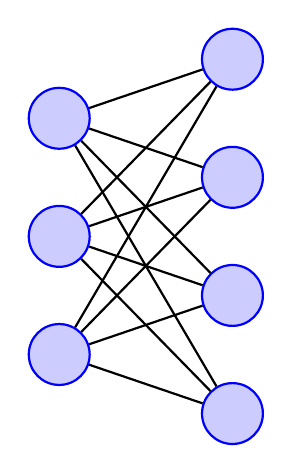
\begin{tikzpicture}[x=2.2cm,y=1.5cm]
		  \readlist\Nnod{3,4} % number of nodes per layer
		  % \Nnodlen = length of \Nnod (i.e. total number of layers)
		  % \Nnod[1] = element (number of nodes) at index 1
		  \foreachitem \N \in \Nnod{ % loop over layers
			% \N     = current element in this iteration (i.e. number of nodes for this layer)
			% \Ncnt  = index of current layer in this iteration
			\foreach \i [evaluate={\x=\Ncnt; \y=\N/2-\i+0.5; \prev=int(\Ncnt-1);}] in {1,...,\N}{ % loop over nodes
			  \node[densenode] (N\Ncnt-\i) at (\x,\y) {};
			  \ifnum\Ncnt>1 % connect to previous layer
				\foreach \j in {1,...,\Nnod[\prev]}{ % loop over nodes in previous layer
				  \draw[thick] (N\prev-\j) -- (N\Ncnt-\i); % connect arrows directly
				}
			  \fi % else: nothing to connect first layer
			}
		  }
		\end{tikzpicture}
	\caption{a Dense Layer}
	\end{figure}
	
	The output value $y_j$ of a dense layer is given by
	$$
	y_j = \sum_{i=1}^{n} x_i w_{i,j} + b_j
	$$
	
	with $b_j$ the bias term for the output neuron $j$
	this equation can be written using matrices
	$$
	Y = XW + B
	$$

	\subsection{Activation layer}

	In a lot of deep neural network content, the activation function is applied inside the dense layer to produce the $y$ output value from the weighted sum $z$.
	but in our implementation, to enhance the seperation of concerns, we opted for a decoupled version.

	\begin{figure}[H]
	\centering
	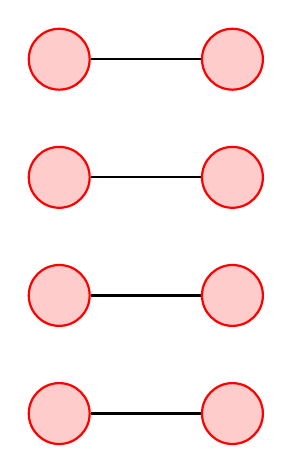
\begin{tikzpicture}[x=2.2cm,y=1.5cm]
	  \readlist\Nnod{4,4} % Define two layers, each with 4 nodes
	  % Loop over both layers
	  \foreachitem \N \in \Nnod{
		\foreach \i [evaluate={\x=\Ncnt; \y=\N/2-\i+0.5; \prev=int(\Ncnt-1);}] in {1,...,\N}{
		  \node[activationnode] (N\Ncnt-\i) at (\x,\y) {};
		  % If not the first layer, connect nodes from the previous layer
		  \ifnum\Ncnt>1
			\draw[thick] (N\prev-\i) -- (N\Ncnt-\i); % Connect nodes element-wise
		  \fi
		}
	  }
	\end{tikzpicture}
	\caption{Element-wise Connections Between Two Layers}
	\end{figure}
	The Activation layer take a vector of size $n$ as input and produce a same length vector as a output, with the activation function applied 
	to each neuron.
	we must note that some activations function transform a vector by mapping individual component through the function, like the ReLU

	$$
	ReLU(z) = max(0, z)
	$$

	while other activation functions such as \textit{softmax} as input a vector $z$ of $K$ real number, 	and is used to convert a vector of $K$ real number into a probability distribution of $K$ possible outcomes.

	$$
	\sigma : \mathbb{R}^{K} \rightarrow (0, 1)^K, K \geq 1
	$$

	is computed by taking a vector $z = (z_1, ..., z_k) \in \mathbb{R}^K$ and compute each component of a vector $\sigma(\mathbf{z}) \in (0, 1)^K$ 

	$$
	\sigma(\mathbf{z})_i = \frac{e^{z_i}}{\sum_{j = 1}^{K} e^{z_j}}
	$$

	we have implemented a variety of activations function, to try out different option and see what works the best with the mnist dataset, more on that in the results section.

	\section{Cost function}
	to mesure how well our neural network perform, we use a cost function, which output a real number, by comparing the neural network \textit{output}, and the effective \textit{observed} value.
	A simple cost function is the meaned squared error, which is defined as : 

	$$
	\text{MSE} = \frac{1}{n} \sum_{i=1}^{n} (\hat{y}_i - y_i)^2
	$$

	this cost function is great for regression neural network, but for a classification task, like the mnist data set (when we need to classifie each image as a digit)
	we can use a cost function like the multi-class cross entropy, which is defined as :
	$$
		\text{Cross Entropy} = -\sum_{c=1}^{C} y_{c} \log(\hat{y}_{c})
	$$

	with $C$ the number of class (eg: 10 for the mnist dataset), $y_{c}$ the observed probability, and $\hat{y}_{c}$ the neural network output.

	and even
	$$
		\text{Cross Entropy (one hot)} = -\log(\hat{y}_{c})
	$$

	as for a one hot encoded observed values vector, only the observed class will be one and every other ocmponent will be 0.

	\section{The learning process}
	
	To make our neural network lean, we want to adjust his parameters (ie: weights and biases) to minimize a cost function $C$.
	The algorithm we used to minimize the cost function is known as \textit{Gradient descent}.
	In a classical gradient descent step, you :

	\begin{enumerate}
		\item feed \textbf{all} your input data points into the network, calculating the cost function for every output.
		\item calculate the overall cost function by averaging each data point cost.
		\item compute the gradient of the overall cost function \textbf{with respect to the network parameters}.
		\item update the parameters
	\end{enumerate}

	\subsection{backpropagation}

	The algorithm used to calculate the gradient of the cost function with respect to the neural network parameters
	is called backpropagation. It is a way to precisely calculate
	(and not only estimate like the finite difference method) this gradient.
	This gradient will be calculated for each layer,
	starting from the last layer and going all the way back to the first layer.
	The key methematical tool used in backpropagation is the chain rule,
	which allow the gradient of the cost function
	to be split into gradient of simpler functions at each neuron within the network.
	For each layer, we want to calculate $\frac{\partial C}{\partial P}$, with $P$ a trainable parameters of the layer,
	we also want to calculate $\frac{\partial C}{\partial X}$ the gradient with respect to input $X$, to be passed to the previous layer.

	\subsection{Dense layer backpropagation}

	The dense layer have two trainable parameters, the weigths, $W$ and the biases $B$.
	Starting with the gradient of the cost function with respect to the weights, we are given
	the output gradient :

	\begin{align}
		\frac{\partial C}{\partial Y} &= \begin{bmatrix}
		\frac{\partial C}{\partial y_1} \\
		\frac{\partial C}{\partial y_2} \\
        \vdots \\
	   \frac{\partial C}{\partial y_j} \\
	\end{bmatrix}
	\end{align}

	The cost function $C$ depend on $Y$ which depend on $W$ thus $C$ depend on $W$

	$$
    \frac{\partial C}{\partial W} = \frac{\partial C}{\partial Y} \frac{\partial Y}{\partial W}
	$$

	We calculate each weight gradient component $\frac{\partial C }{\partial W_{ij}}$

	$$
    \frac{\partial C}{\partial W_{ij}} = \sum_{l=1}^{N} \frac{\partial L}{\partial Y_{lj}} \frac{\partial Y_{lj}}{\partial W_{ij}}
	$$

	because $W_{ij}$ is used in every example for calculating the $j^{th}$ column of the output matrix. Let's look at the formula for $Y_{lj}$ to get the derivative

	$$
		Y_{lj} = X_{l1}W_{1j} + \cdots + X_{li}W_{ij} + \cdots + X_{lp}W_{pj} + b_{j}
	$$
	$$
		\frac{\partial Y_{lj}}{\partial W_{ij}} = X_{li}
	$$
	$$
		\implies \frac{\partial C}{\partial W_{ij}} = \sum_{l=1}^{N} \frac{\partial C}{\partial Y_{lj}} X_{li} = \sum_{l=1}^{N} X^{T}_{il}\frac{\partial C}{\partial Y_{lj}}
	$$

	So finally 

	$$
		\frac{\partial C}{\partial W} = X^{T} \frac{\partial C}{dY}
	$$

	for the biases $B$.

	\begin{align}
		\frac{\partial C}{\partial b} &= \frac{\partial C}{\partial Y} \frac{\partial Y}{\partial b}\\
		\frac{\partial C}{\partial b_{i}} &= \sum_{l=1}^{N} \frac{\partial C}{\partial Y_{li}} \frac{\partial Y_{li}}{db}
	\end{align}

	since the bias term $b_{i}$ is used in the evaluation of the entire column of $Y$.

	$$
		\frac{\partial Y_{li}}{\partial b_{i}} = 1
	$$
	$$
		\frac{\partial C}{db_{i}} = \sum_{l=1}^{N} \frac{\partial C}{\partial Y_{li}}
	$$
	$$
		\frac{\partial C}{\partial b} = \frac{\partial C}{\partial Y}
	$$

	and lastly, we calculate the gradient with respect to $X$

	\begin{align}
		\frac{\partial C}{\partial X} &= \frac{\partial C}{\partial Y} \frac{\partial Y}{\partial X}\\
		\frac{\partial C}{\partial X_{ij}} &= \sum_{l=1}^{k} \frac{\partial C}{\partial Y_{il}} \frac{\partial Y_{il}}{\partial X_{ij}}
	\end{align}

	since the data point $i$ will only influence the data point $i$ in $Y$. Other data points will not be affected. Further, $X_{ij}$ is used in calculation of every dimension of $Y_{i,:}$. To calculate the gradient,

	$$
		Y_{il} = \sum_{t=1}^{p} X_{it}W_{tl}
	$$
	$$
		\frac{\partial Y_{il}}{\partial X_{ij}} = W_{jl}
	$$
	$$
		\frac{\partial C}{\partial X_{ij}} = \sum_{l=1}^{k} \frac{\partial C}{\partial Y_{il}}W_{jl}
		= \sum_{l=1}^{k} \frac{\partial C}{\partial Y_{il}} W_{lj}^{T}
	$$
	$$
		\implies \frac{\partial C}{\partial X} = \frac{\partial C}{\partial Y} W^{T}
	$$

	\subsection{Activation layer backpropagation}

	An activation layer doesn't have any trainable parameters, so we just gonna focus on the input gradient calculation.

	we are given
	the output gradient $\frac{\partial C}{\partial Y}$:
	we know that 

	\begin{align*}
		Y &= \begin{bmatrix}
		f(X_1) \\
		f(X_2) \\
        \vdots \\
		f(X_i)
	\end{bmatrix}
	\end{align*}

	$$
    \frac{\partial C}{\partial X} = \frac{\partial C}{\partial Y} \frac{\partial Y}{\partial X}
	$$

	$$
    \frac{\partial C}{\partial X_{ij}} = \sum_{l=1}^{N} \frac{\partial C}{\partial Y_{lj}} \frac{\partial Y_{lj}}{\partial X_{ij}}
	$$

	using the same procedure as for the previous calculations

	$$
	\implies \frac{\partial C}{\partial X} = \frac{\partial C}{\partial Y} \odot Y\prime
	$$

	with 

	\begin{align*}
		Y\prime &= \begin{bmatrix}
		f\prime(X_1) \\
		f\prime(X_2) \\
        \vdots \\
		f\prime(X_i)
	\end{bmatrix}
	\end{align*}

	\section{Optimizers}
	
	At this point, to updates a neural network parameter $\theta$, we the gradient descent formula,
	with a fix learning rate $\eta$

	$$
	\theta := \theta - \eta \frac{\partial C}{\partial \theta}
	$$

	This is know, in the keras api for exemple as the \textit{Stochastic gradient descent optimizer},
	but it exist other optimizers such as \textit{Adam}.

	\subsection{Adam}
	Adam accelerate the convergence towards the optimal set of weights by taking into account pass gradient,
	and adam will adapt the learning rate for each individual weight.

	ADAM initializes two vectors, 
	$m$ and $v$, which store the exponential moving averages of past gradients and past squared gradients,
	respectively. These vectors are used to scale the gradient updates adaptatively.

	\begin{enumerate}
	  \item \textbf{Initialization:} Initialize two vectors, $m$ and $v$, to store the moving averages of the gradients and their squares, respectively.
	  \item \textbf{Computing Moving Averages of the Gradients:}
		\begin{align*}
		  m_t &= \beta_1 \cdot m_{t-1} + (1 - \beta_1) \cdot g_t, \\
		  v_t &= \beta_2 \cdot v_{t-1} + (1 - \beta_2) \cdot g_t^2,
		\end{align*}
		where $g_t$ is the gradient at time step $t$, and $\beta_1$ and $\beta_2$ are factors that control the decay rates.
	  \item \textbf{Bias Correction:} Correct initial bias in $m$ and $v$:
		\begin{align*}
		  \hat{m}_t &= \frac{m_t}{1 - \beta_1^t}, \\
		  \hat{v}_t &= \frac{v_t}{1 - \beta_2^t}.
		\end{align*}
	  \item \textbf{Update Weights:} Adjust weights based on the corrected moments:
		\begin{equation*}
		  \theta_{t+1} = \theta_t - \frac{\eta}{\sqrt{\hat{v}_t} + \epsilon} \cdot \hat{m}_t,
		\end{equation*}
		where $\theta$ are the parameters, $\eta$ is the learning rate, and $\epsilon$ is a small constant for numerical stability.
	\end{enumerate}

	\section{All about batch}
	We went through several feed forward implementations. The first one was to pass data point one by one in the network
	$x \in \mathbb{R}^{i}$\dots. This was very slow, for exemple, for the mnist dataset, which has 60k training exemples,
	we where going through the whole neural network : feed forward, cost evaluation, back propagation, 60k times.
	But we then leraned that we can instead pass \textit{batch} of data in the neural network, in one time, and this batch can
	be of any length.
	the input then becomes $x \in M_{nxi} (\mathbb{R})$ with each line of the input matrice representing a single data point.

	The calculation became much faster, because we can now feed $n$ element at a time in the neural network.

	\section{Initializer}
	
	\section{Convolutional neural network}
	ALEXIS a toi de travailler

	\section{Metrics}
	
	\section{Training, Validation and Test}
	To monitor the performances of our neural network, it is important to break down our 

	To measure how well the neural network has performed over our dataset, we can calculate multiple metrics, the first one, that we already have in hand
	is the cost.

	\section{Results}
	With our library, we can declarativaly create neural network, we are gonna list once the code to declare a net, and describe it.

	\begin{minted}[breaklines, tabsize=2]{rust}
let net = NeuralNetworkBuilder::new()
	.watch(MetricsType::Accuracy)
	.push(DenseLayer::new(
		28 * 28,
		32,
		InitializerType::GlorotUniform,
	))
	.push(
		ActivationLayer::from(Activation::ReLU)
	)
	.push(
		DenseLayer::new(32, 10, InitializerType::GlorotUniform)
	)
	.push(
		ActivationLayer::from(
			Activation::Softmax
		)
	);
Ok(net.compile(GradientDescent::new(0.01), CostFunction::CrossEntropy)?)
	\end{minted}

	here we have defined a neural network with only one hidden layer, containing 32 neuron.
	we have initialized our weights with the Glorot uniform method, and used the ReLU activation function after the hidden layer
	after the output layer, we have normalized the logits with the softmax function, and used cross entropy cost function.

	in our library, you can use the \textit{watch} method to watch a \textit{MetricsType}, here we watched the accuracy of the network
	this will give us the network accuracy, with the training, validation and test set.

	throughout the analysis of the results, to reach for the best neural network, we will try to reach the \textit{VC trade-off principle} \cite{LeCun2019} \cite{vapnik1974theory},
	this principle explain that:

	\begin{enumerate}
		\item A more complex model might fit the training data very well (low training error) but risks overfitting, meaning it could perform poorly on new data because it is too tailored to the training set (high variance).
		\item A less complex model might not fit the training data as closely (higher training error) but can generalize better on new data because it does not capture the noise and specific details of the training set (low variance).
	\end{enumerate}

	Our challenge will thus be, to find the right level of complexity that minimizes both the error on the training data and the error on unseen data.
	We will often start with a low complexity model, and try to lift the complexity up unitl we met overfitting.

	\subsection{Multi-layer perceptron}

	for a simple sequential neural network, wiith one hidden layer of 32 neuron.


	\begin{table}[H]
	\centering
	\begin{tabular}{|l|c|c|c|c|c|}
	\hline
	Parameters & epochs & batch size  \\
	\hline
	Value & 15 & 128   \\
	\hline
	\end{tabular}
	\caption{Table 1 of the \textbf{original article} comparing MSE values for various denoising algorithms}
	\end{table}

	\subsection{Convolutional multi-layer perceptron}

	\section{Optimisations}
	vérifier que l'interpretation du flamegrpah est correct et que je dis pas de la merde.

	In additions to batching, to further optimize our rust code, we can look at the flamegraph of our functions call, 

	\section{Discussion}

	\section{Conclusion}

	\printbibliography

\end{document}
